\section{Wallet}
Il wallet consente la gestione di credenziali richieste presso un issuer.

\subsection{Registrazione al Wallet}
Per la registrazione occorre fornire un indirizzo email e una password
\begin{center}
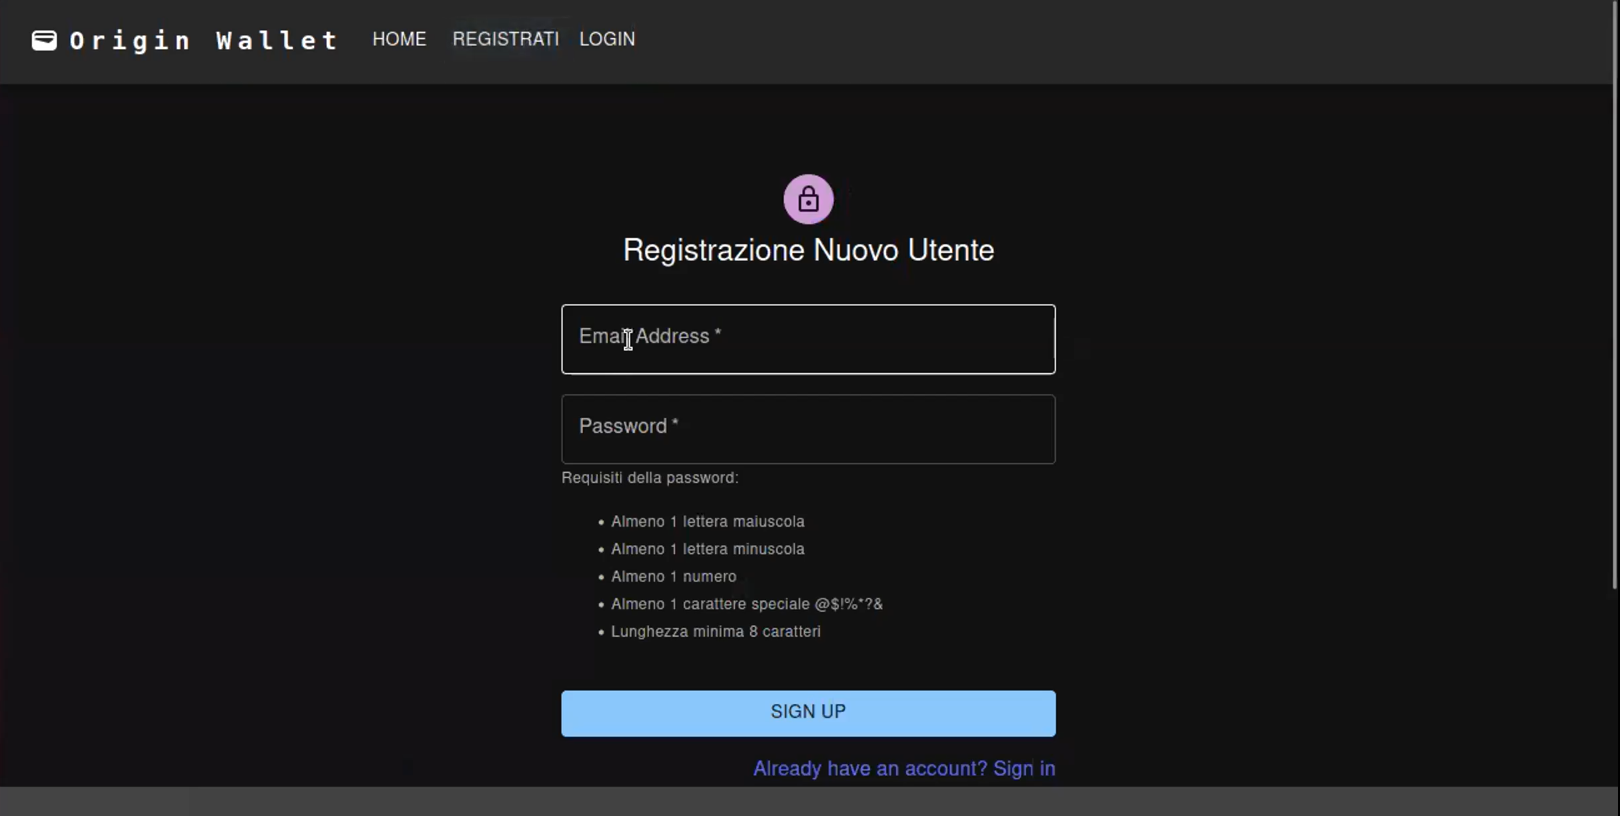
\includegraphics[scale = 0.9]{./res/img/wallet/wallet_register.png}
\end{center}

\subsection{Login al Wallet}
Il login si effettua utilizzando email e password utilizzate durante la registrazione

\subsection{Storage di credenziale}
Una volta effettuato il login al wallet e richiesto il Rilascio di una credenziale presso un issuer, è possibile concludere il processo di Issuing cliccando su Accept.\\
In questo modo la credenziale verrà memorizzata nel wallet
\begin{center}
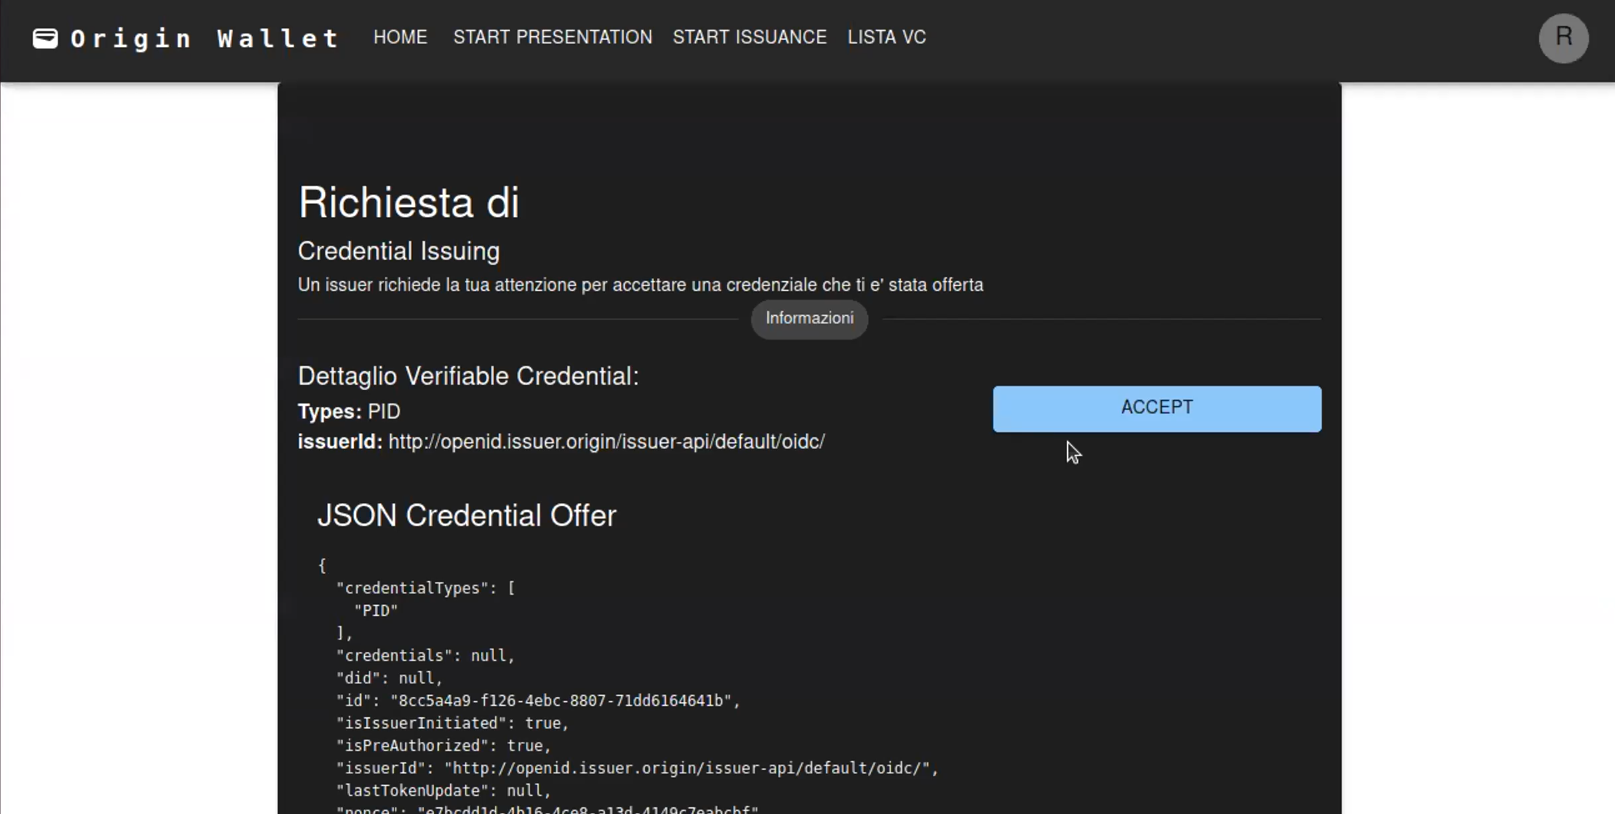
\includegraphics[scale = 0.9]{./res/img/wallet/wallet_continue_issuing.png}
\end{center}

\subsection{Presentazione di credenziale}
Cliccando su START PRESENTATION è possibile presentare una credenziale ad un verifier per poter accedere a dei servizi
\begin{center}
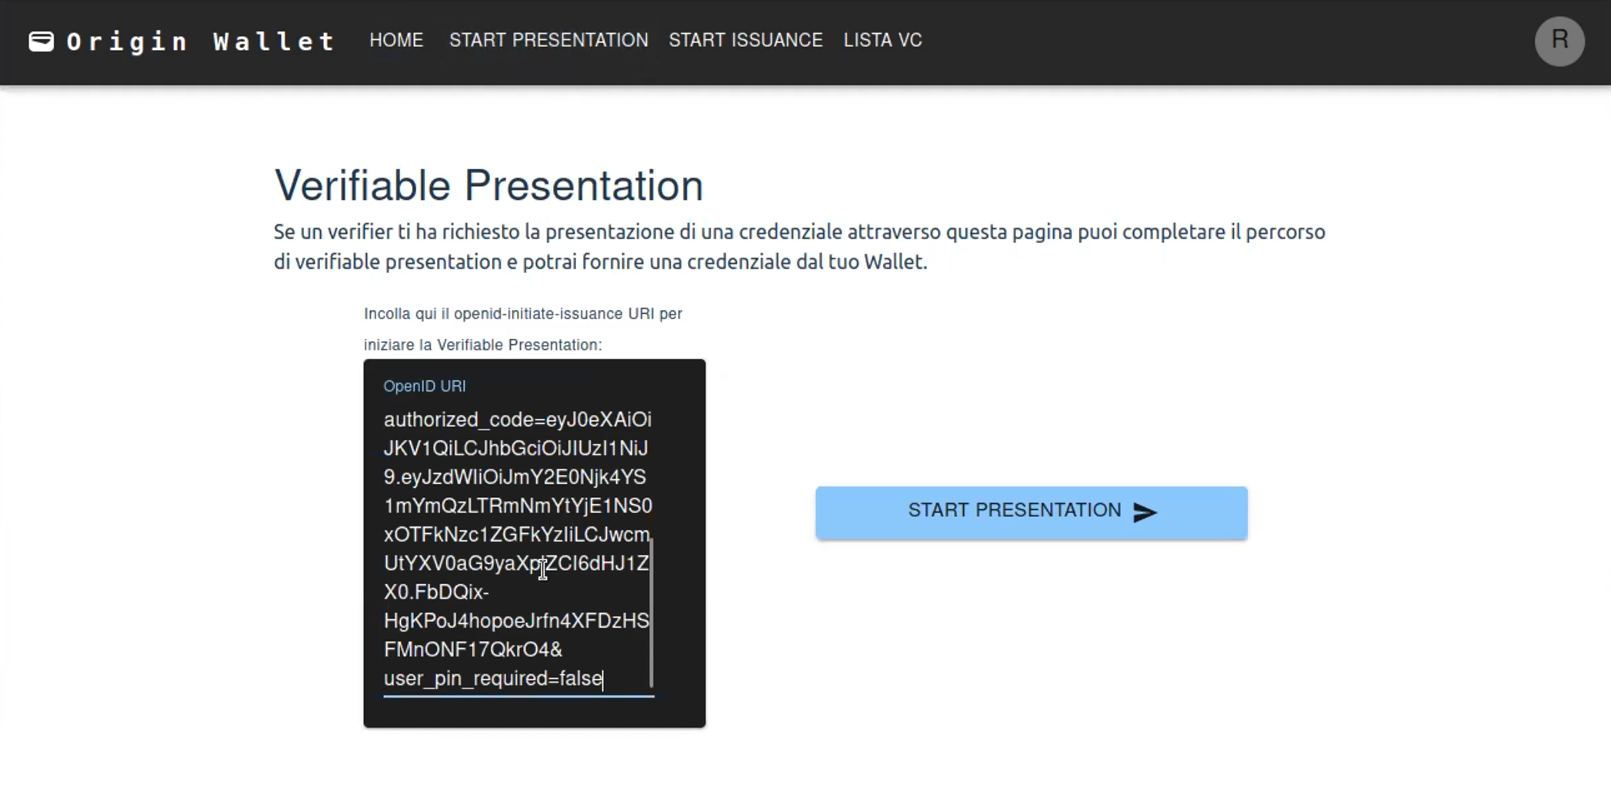
\includegraphics[scale = 0.9]{./res/img/wallet/wallet_start_presentation.png}
\end{center}
\subsection{Visualizzazione e gestione}
Nella pagina di visualizzazione verrà mostrato un elenco di tutte le credenziali memorizzate nel wallet. \newline
\begin{center}
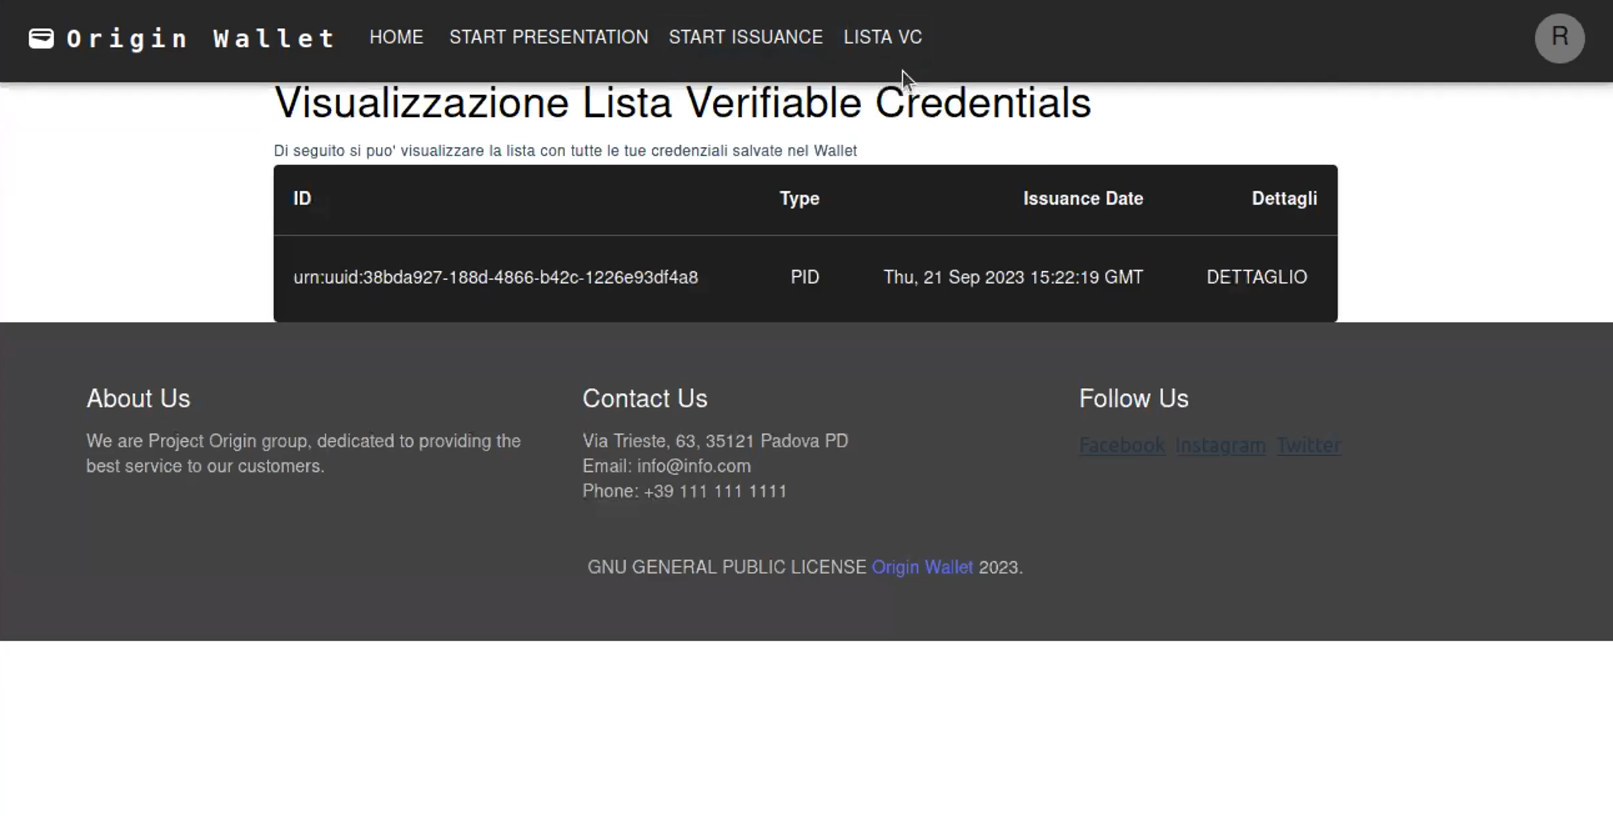
\includegraphics[scale = 0.9]{./res/img/wallet/wallet_credentials_list.png}
\end{center}
Cliccando su DETTAGLIO è possibile visualizzare tutte le informazioni memorizzate nella credenziale. \\
\begin{center}
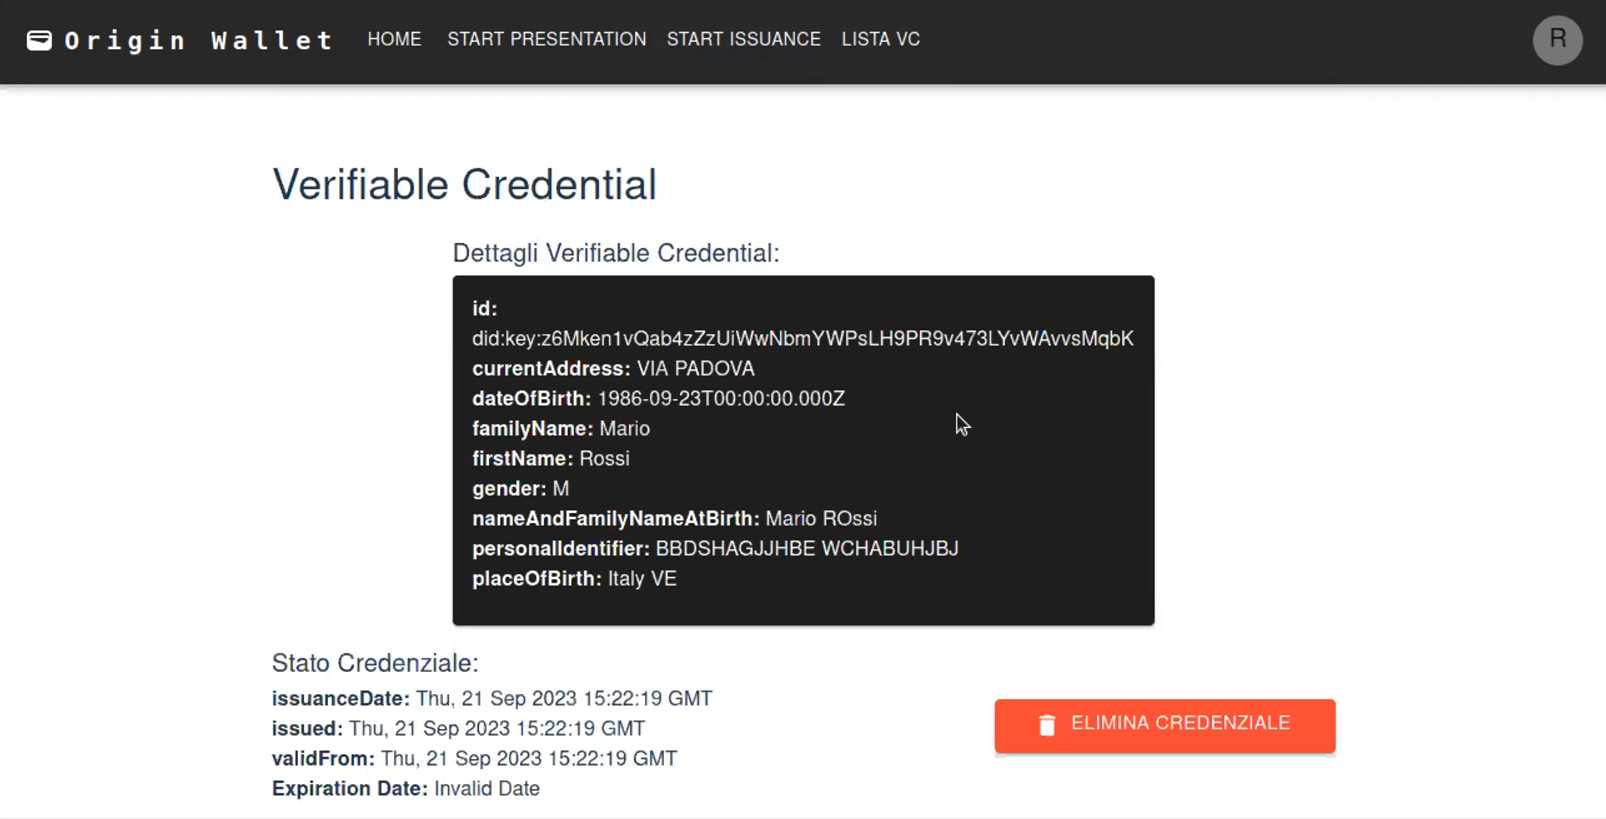
\includegraphics[scale = 0.9]{./res/img/wallet/wallet_credential_detail.png}
\end{center}
In seguito è possibile visualizzate tutte le informazioni contenute in una credenziale, e si può decidere di eliminarla.
\begin{center}
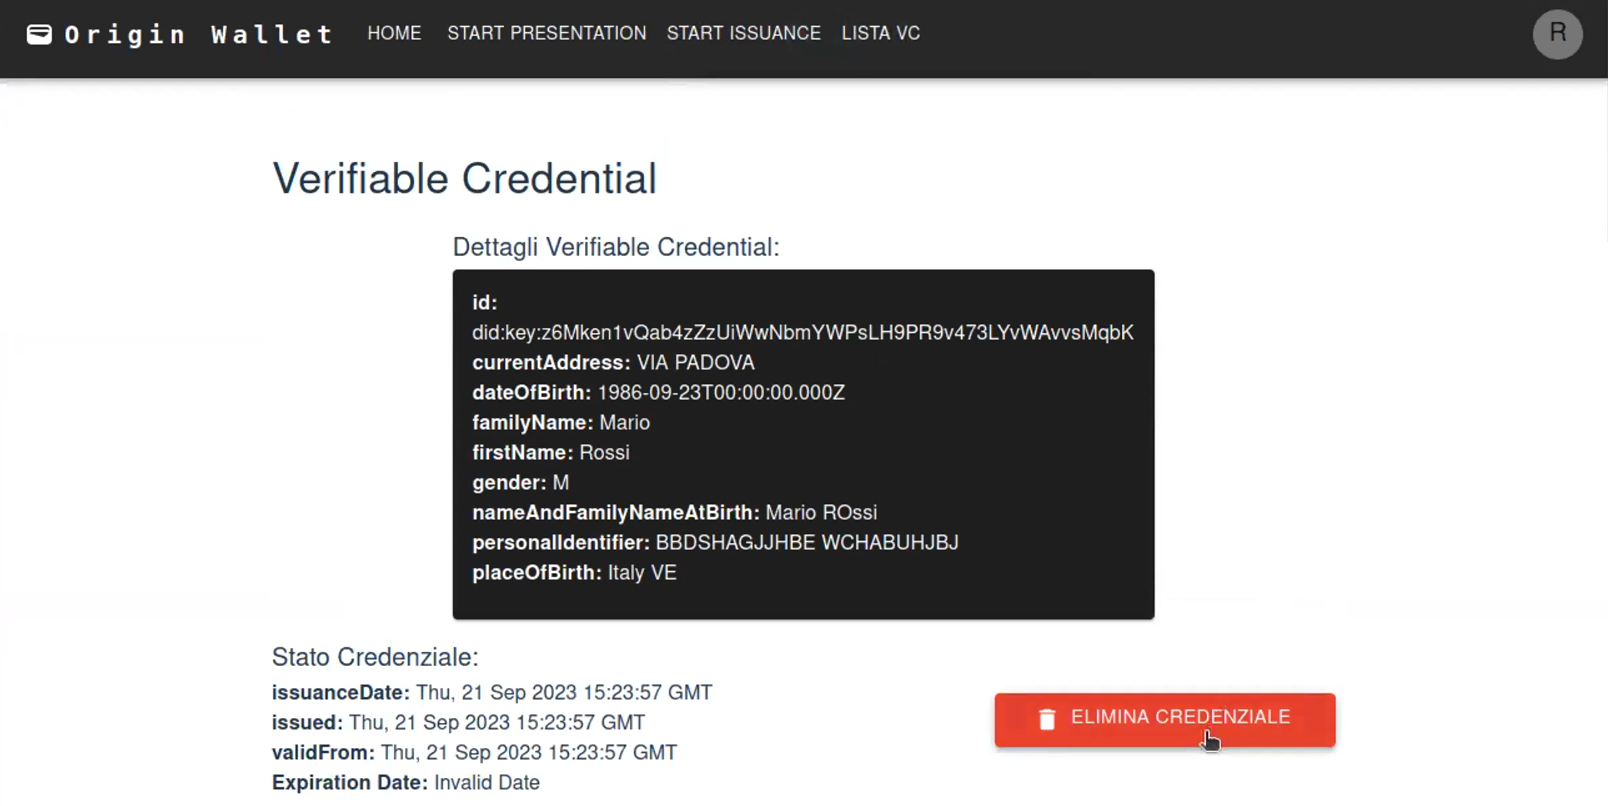
\includegraphics[scale = 0.9]{./res/img/wallet/wallet_credential_delete.png}
\end{center}
%anche se questa immagine è quasi identica a quella di prima, la lascerei